% !TeX program = xelatex
\documentclass[tikz,border=5pt]{standalone}
\usepackage{fontspec}
\usepackage{unicode-math}
\setmainfont{Times New Roman}
\setmathfont{texgyretermes-math.otf}
\usetikzlibrary{arrows.meta,positioning,calc}

\definecolor{ink}{HTML}{25272A}
\definecolor{muted}{HTML}{6F747A}
\definecolor{rule}{HTML}{B9BEC4}
\definecolor{wash}{HTML}{F3F5F7}

\begin{document}
% Coordinate ledger (replace before drawing):
% target width = ... mm
% columns x = ...
% rows y = ...
% standard node size = ...
% routing lanes = ...
% solid frame = core / observed / directly modeled
% dashed frame = auxiliary / derived / copied / intermediate / contextual
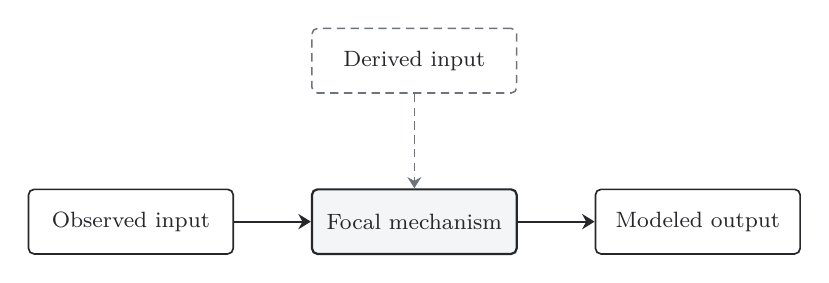
\begin{tikzpicture}[
  font=\rmfamily,
  >=Stealth,
  labeltext/.style={font=\rmfamily\fontsize{8}{9}\selectfont,text=ink},
  annotation/.style={font=\rmfamily\fontsize{7}{8}\selectfont,text=muted},
  box/.style={draw=ink,line width=.6pt,fill=white,rounded corners=2pt,
    minimum width=2.6cm,minimum height=.82cm,inner sep=5pt,align=center,
    font=\rmfamily\fontsize{8}{9}\selectfont,text=ink},
  auxiliary/.style={box,draw=muted,line width=.55pt,dash pattern=on 3pt off 2pt},
  context/.style={box,draw=rule,fill=wash,line width=.5pt},
  focal/.style={box,draw=ink,line width=.8pt,fill=wash},
  primary/.style={-{Stealth[length=4.5pt,width=5.5pt]},draw=ink,line width=.75pt},
  copy/.style={-{Stealth[length=4pt,width=5pt]},draw=muted,line width=.55pt,
    dash pattern=on 3pt off 2pt},
  dependency/.style={-{Stealth[length=4pt,width=5pt]},draw=muted,line width=.55pt,
    dash pattern=on .8pt off 1.7pt},
  separator/.style={draw=rule,line width=.45pt}
]

% Replace this skeleton with the method- and benchmark-driven layout.
\node[box] (input) at (0,0) {Observed input};
\node[focal] (process) at (3.6,0) {Focal mechanism};
\node[box] (output) at (7.2,0) {Modeled output};
\node[auxiliary,above=1.2cm of process] (aux) {Derived input};
\draw[primary] (input.east) -- (process.west);
\draw[copy] (aux.south) -- (process.north);
\draw[primary] (process.east) -- (output.west);

\end{tikzpicture}
\end{document}
